% !TEX TS-program = XeLaTeX
% use the following command:
% all document files must be coded in UTF-8
\documentclass[english]{textolivre}
% build HTML with: make4ht -e build.lua -c textolivre.cfg -x -u article "fn-in,svg,pic-align"

\journalname{Texto Livre}
\thevolume{15}
%\thenumber{1} % old template
\theyear{2022}
\receiveddate{\DTMdisplaydate{2022}{7}{17}{-1}} % YYYY MM DD
\accepteddate{\DTMdisplaydate{2022}{8}{1}{-1}}
\publisheddate{\DTMdisplaydate{2022}{9}{21}{-1}}
\corrauthor{Borja Fernández García-Valdecasas}
\articledoi{10.35699/1983-3652.2022.40505}
%\articleid{NNNN} % if the article ID is not the last 5 numbers of its DOI, provide it using \articleid{} commmand 
% list of available sesscions in the journal: articles, dossier, reports, essays, reviews, interviews, editorial
\articlesessionname{dossier}
\runningauthor{García-Valdecasas et al.} 
%\editorname{Leonardo Araújo} % old template
\sectioneditorname{Daniervelin Pereira}
\layouteditorname{Carolina Garcia}

\title{Role of neurodidactics in teacher professionalization for online teaching in higher education}
\othertitle{O papel da neurodidáctica na profissionalização de professores para ensino \textit{online} na educação superior}
% if there is a third language title, add here:
%\othertitle{Artikelvorlage zur Einreichung beim Texto Livre Journal}

\author[1]{Borja Fernández García-Valdecasas~\orcid{0000-0002-1851-6596}\thanks{Email: \href{mailto:borjagv@correo.ugr.es}{borjagv@correo.ugr.es}}}
\author[2]{Isabel Martínez Sánchez~\orcid{0000-0003-0802-4878}\thanks{Email: \href{mailto:imsanchez@edu.uned.es}{imsanchez@edu.uned.es}}}
\author[3]{Daniel González González~\orcid{0000-0001-7311-5819}\thanks{Email: \href{mailto:danielg@ugr.es}{danielg@ugr.es}}}
\author[4]{José Álvarez Rodríguez~\orcid{0000-0002-8411-9265}\thanks{Email: \href{mailto:alvarez@ugr.es}{alvarez@ugr.es}}}
\affil[1]{Universidad de Nebrija, Facultad de Lenguas y Educación, Departamento de Educación, Madrid, España.}
\affil[2]{Universidad Nacional de Educación a Distancia, Facultad de Educación, Departamento MIDE, Madrid, España.}
\affil[3]{Universidad de Granada, Facultad de Ciencias de la Educación, Departamento de MIDE, Granada, España.}
\affil[4]{Universidad de Granada, Facultad de Ciencias de la Educación, Departamento de Pedagogía, Granada, España.}


\addbibresource{article.bib}
% use biber instead of bibtex
% $ biber article

% used to create dummy text for the template file
\definecolor{dark-gray}{gray}{0.35} % color used to display dummy texts
\usepackage{lipsum}
\SetLipsumParListSurrounders{\colorlet{oldcolor}{.}\color{dark-gray}}{\color{oldcolor}}

% used here only to provide the XeLaTeX and BibTeX logos
\usepackage{hologo}

% if you use multirows in a table, include the multirow package
\usepackage{multirow}

% provides sidewaysfigure environment
\usepackage{rotating}

% CUSTOM EPIGRAPH - BEGIN 
%%% https://tex.stackexchange.com/questions/193178/specific-epigraph-style
\usepackage{epigraph}
\renewcommand\textflush{flushright}
\makeatletter
\newlength\epitextskip
\pretocmd{\@epitext}{\em}{}{}
\apptocmd{\@epitext}{\em}{}{}
\patchcmd{\epigraph}{\@epitext{#1}\\}{\@epitext{#1}\\[\epitextskip]}{}{}
\makeatother
\setlength\epigraphrule{0pt}
\setlength\epitextskip{0.5ex}
\setlength\epigraphwidth{.7\textwidth}
% CUSTOM EPIGRAPH - END

% LANGUAGE - BEGIN
% ARABIC
% for languages that use special fonts, you must provide the typeface that will be used
% \setotherlanguage{arabic}
% \newfontfamily\arabicfont[Script=Arabic]{Amiri}
% \newfontfamily\arabicfontsf[Script=Arabic]{Amiri}
% \newfontfamily\arabicfonttt[Script=Arabic]{Amiri}
%
% in the article, to add arabic text use: \textlang{arabic}{ ... }
%
% RUSSIAN
% for russian text we also need to define fonts with support for Cyrillic script
% \usepackage{fontspec}
% \setotherlanguage{russian}
% \newfontfamily\cyrillicfont{Times New Roman}
% \newfontfamily\cyrillicfontsf{Times New Roman}[Script=Cyrillic]
% \newfontfamily\cyrillicfonttt{Times New Roman}[Script=Cyrillic]
%
% in the text use \begin{russian} ... \end{russian}
% LANGUAGE - END

% EMOJIS - BEGIN
% to use emoticons in your manuscript
% https://stackoverflow.com/questions/190145/how-to-insert-emoticons-in-latex/57076064
% using font Symbola, which has full support
% the font may be downloaded at:
% https://dn-works.com/ufas/
% add to preamble:
% \newfontfamily\Symbola{Symbola}
% in the text use:
% {\Symbola }
% EMOJIS - END

% LABEL REFERENCE TO DESCRIPTIVE LIST - BEGIN
% reference itens in a descriptive list using their labels instead of numbers
% insert the code below in the preambule:
%\makeatletter
%\let\orgdescriptionlabel\descriptionlabel
%\renewcommand*{\descriptionlabel}[1]{%
%  \let\orglabel\label
%  \let\label\@gobble
%  \phantomsection
%  \edef\@currentlabel{#1\unskip}%
%  \let\label\orglabel
%  \orgdescriptionlabel{#1}%
%}
%\makeatother
%
% in your document, use as illustraded here:
%\begin{description}
%  \item[first\label{itm1}] this is only an example;
%  % ...  add more items
%\end{description}
% LABEL REFERENCE TO DESCRIPTIVE LIST - END


% add line numbers for submission
%\usepackage{lineno}
%\linenumbers

\begin{document}
\maketitle

\begin{polyabstract}
\begin{abstract}
The objective of this article is to perform a bibliometric analysis that helps to delimit and understand the concepts of Neuroscience and Neurodidactics, taught in higher education, for a better understanding of the different learning processes, that is, to try to explain what, how and why we learn. A quantitative-bibliometric methodology was employed using the Web of Science (WoS) database. The search was performed by filtering "subject and key terms" in both titles and abstracts of scientific papers using Boolean operators and truncations. We proceeded to work with two samples: the first one without using any kind of filter or refinement of 60 scientific papers; the second one filtering by the thematic categories with a sample of 44 scientific papers.  The years of production, the sources of information, the authors and the keywords of the scientific documents were considered for the analysis of the data. From the results shown through the maps, a total of five research fronts have been inferred as the most relevant and related to the topic: neurodidactics in general; neuroscience and technology; neurodidactics and technological aspects; neuroeducation programs and pedagogy and neurodidactics. As this is a developing field of study, no major specific problems have been found, but for the time being what is obtained is a  broad and general view of this area of research. Future studies that complement or expand this work could be oriented towards conducting replication research.

\keywords{Bibliometrics \sep Neuroscience \sep Neuroeducation \sep Neurodidactics \sep Technology}
\end{abstract}

\begin{portuguese}
\begin{abstract}
O objetivo deste artigo é realizar uma análise bibliométrica que ajude a delimitar e compreender os conceitos de Neurociência e  Neurodidática, ensinados no ensino superior, para uma melhor compreensão dos diferentes processos de aprendizagem, ou seja, tentar explicar o quê, como e por que aprendemos. Foi utilizada uma metodologia quantitativo-bibliométrica a partir da base de dados da Web of Science (WoS). A pesquisa foi realizada por meio da filtragem por "assunto e termos chave" tanto em títulos como em resumos de artigos científicos, utilizando operadores booleanos e truncamentos. Procedemos ao trabalho com duas amostras: a primeira sem utilizar qualquer tipo de filtro ou refinamento de 60 artigos científicos; a segunda filtrando pelas categorias temáticas com uma amostra de 44 artigos científicos. Para a análise dos dados, foram considerados os anos de produção, as fontes de informação, os autores e as palavras-chave dos documentos científicos. Dos resultados apresentados através dos mapas, inferiu-se um total de cinco frentes de investigação como as mais relevantes e relacionadas com o tema, tais como: neurodidática em geral; neurociência e tecnologia; neurodidática e aspectos tecnológicos; programas de neuroeducação e pedagogia e neurodidática. Como se trata de um campo de estudo em desenvolvimento, não foram encontrados grandes problemas específicos, mas, por enquanto, o que se obtém é uma visão bastante ampla e geral dessa área de investigação. Estudos futuros que complementem ou expandam este trabalho poderiam ser orientados para a realização de investigação de replicação.

\keywords{Bibliometria \sep Neurociência \sep Neuroeducação \sep Neurodidática \sep Tecnologia}
\end{abstract}
\end{portuguese}
% if there is another abstract, insert it here using the same scheme
\end{polyabstract}

\section{Introduction}

One of the essential questions we must determine in this first approach is to be able to delimit and understand what means neuroscience. The word “neuroscience” is understood as the union of a wide and diverse conjunction of sciences, whose objective is to make known and therefore, to understand the composition, structure and different functions of our nervous system and therefore our brain \cite{cavada_como_2012}. This concept was created in 1969 with the creation of the "Society of Neuroscience" and, years later, in 1985 in Spain, the Spanish Society of Neuroscience \cite{morgado-bernal_frequency_2011}.

The concept of neuroscience is composed of two fundamental elements: neuro which means nerve; and science whose meaning implies knowledge. Neuroscience, when applied to human beings, analyzes the nervous system and its interaction of the various elements causing biological bases of behavior. In order to understand the complexity of the concept of neuroscience, it is supported by philosophy, since its purpose is to know man in a holistic way. Neuroscience attempts to explain how millions of individual nerve cells in the brain act to produce behavior and how, in turn, these cells are influenced by the environment, including the behavior of other individuals \cite{salas_silva_educacion_2003}. Neuroscience understands learning as any change in the synaptic connections that cause variations in thought and behavior produced by theoretical information, practice or life experiences.

Looking from neurodidactics \cite{unzueta_educacion_2011}, he states that the main need to obtain knowledge is emotion. It is through emotion that curiosity is stimulated continuing later with the stimulation of attention activating neural mechanisms of learning and memory \cite{mora_dios_2014,benavidez__importancia_2019}.

Several authors such as \textcite{ortiz_aportes_2018}, define neurodidactics as:
\begin{quote}
    "A branch of neuroscience that through the knowledge of the neurophysiology of mental processes, aims to design teaching strategies for teachers and learning strategies for students, effectively and efficiently, with the objective of promoting greater brain development, and with this improve teaching practice and at the same time the development of permanent competencies in students." \cite[p.~10]{ortiz_aportes_2018}.
\end{quote}
	
This definition proposes the understanding of the different learning processes, that is, it tries to explain what, how and why we learn, delimiting the way in which we do it, giving great importance to the senses and cognitive abilities.

Neurodidactics is a discipline that analyzes the optimization of the teaching and learning process based on the development process of the brain (with all the neuronal potential) \cite{alarcon_neurodidactica_2020}.

\section{Towards a neurodidactic approach}

The educational methodology that arises from the great advances in neuroscience is neurodidactics. It is in charge of analyzing the cerebral bases of the teaching processes (the teaching-learning process, the different strategies so that, within a class, significant learning takes place). This learning strategy is based on some principles such as: the main role is played by the student, who plays an active role in learning, his interests and needs, emotional character, his way of studying, his reasoning and understanding.
Some methods to carry out neurodidactics in the classroom are:

\begin{itemize}
    \item Invert the traditional classroom mode.
    \item Group learning.
    \item Frequent use of new technologies.
    \item Flexibility of schedules and use of various methods, groupings \cite{muchiut_neurodidactica_2018}.
\end{itemize}

In the following lines, we will delve into some important agents for an effective development of neurodidactics in education. The first of these is to give students total freedom both in and out of the classroom. This lowers stress levels and improves student performance. In addition, it is necessary to promote very specific cognitive skills such as art, reading or meditation inducing neurogenesis in the brain, causing a positive impact on learning.  The teacher will always have to take into account the individual characteristics, talents and interests of each of the students. Good learning induces to it.

The plasticity of the brain \cite{rebolledo_plasticidad_2003,aguilar_plasticidad_2003}, allows the student to adapt to the circumstances and new events of the teaching-learning process, requiring constant practice of the contents. In short, neurodidactics is the result of the convergence of psychology, pedagogy and neuroeducation.

From these approaches, \textcite{machicado_mamani_neurodidactica_2015}, state that: 

\begin{quote}
"Neurodidactic strategies are ideal modalities designed, adapted and executed by the teacher, according to the profile of the career, the context, the pace and learning style of students, under flexible and self-flexible cooperative schemes, susceptible to be applied in teacher training." \cite[p.~51]{machicado_mamani_neurodidactica_2015} 
\end{quote}

These same researchers cite some neurodidactic approaches to the teaching-learning process, including:

\begin{itemize}
    \item Operational: A set of creative forms of teaching created according to the interest of the learner and the context in which he/she finds himself/herself. For example, we highlight: maieutics, mnemonics, metaphor, analogy, previous organizers, interaction tactics \cite{_cusme_estrategias_2021}.
\end{itemize}

We will now proceed to explain each of them in the following lines. In the first place, maieutics is the learning that takes place through questions, that is, the learner is questioned and then put in the process of debating his answer, making him arrive at knowledge through his own conclusions and not simply through learned or pre-conceptualized knowledge. Mnemonics is the associative process of remembering or memorizing knowledge, such as images, words or phrases. Some examples of mnemonic rules are acronyms, phrases, rhymes or melodies, fragments and stories.Thirdly, metaphor is, in short, the establishment of links between two things that are apparently different but share some common feature. On the other hand, analogy is the juxtaposition of two or more objects or experiences that share general and specific characteristics. Thus, reasoning and behaviors will be established taking into account the similarities between them. This allows the acquisition of new knowledge, development of mental and creative capacity, imagination and cognitive fluency.

Another strategy is the interaction tactics, content-student, teacher-student, student-student within the educational environment, for example: the space in which they live and coexist, exchanges of impressions and opinions and, finally, reactions that educational actors generate. One of the most innovative forms is ICT, which helps in the construction of educational learning.

Finally, we will talk about previous organizers, which are a very useful instructional resource for meaningful learning, since they help to establish previous knowledge, thus achieving the acquisition of knowledge.

\section{Teaching and learning in Higher Education}

Learning in the adult stage has some unique characteristics \cite{anaya_exito_2014}, which comes from psychological particularities of adulthood, to the places where it increases reaching the contents that are undertaken at each stage \cite{vergel-ortega_factores_2016}. \textcite{unesco_educacion_2005} refers to the process of adult education as the pursuit of achieving a rational and autonomous state capable of being applied to data of objective nature. This type of education focuses on the appropriation, regardless of age, of attitudes and aptitudes that are prone to the blurring of communication processes.

In terms of sociology, adults are perfectly included in the social environment, possessing full rights, freedoms and responsibilities. Regarding the psychological aspects, it is a more difficult question. The word "adult" is used as a synonym for personal maturity, adult in his full mental faculties, fullness of judgment, seriousness and mastery of emotions. The learning capacity of adults, including and focusing on older people, is substantially influenced by training, motivation and the learning situation, which must be favorable \cite{cuenca_motivacion_2011}.
	
Intrapersonal motives can influence the development of the teaching-learning process \cite{cadena_narvaez_incidencia_2016,jimenez_climent_inteligencias_2017}:

\begin{enumerate}
    \item Cognitive styles of the individual.
    \item Their learning methodologies and autonomous intellectual work.
    \item Personality, control of emotions and self-concept anxiety.
    \item Motivation \cite{martinez_lopez_salud_2003,fernandez_palacio_neurodidactica_2017}.
\end{enumerate}

In the field of adult education, we have to eliminate any behavior related to learning that is set in an authoritarian way. It is recommended that the adult learner establishes his or her learning and educational processes. Some subjects will need orientation guidelines.

Some conditions that we must keep in mind in adult learning:

\begin{itemize}
    \item Comfort in learning by creating an atmosphere conducive to learning.
    \item Obligations external to learning (housework, transportation, childcare, etc.), influencing their learning.
\end{itemize}

Below we show the analyses carried out in one of the most important databases, such as the Web of Science (WoS), to determine the number of scientific contributions, which include the terms "Neuroscience, Neurodidactics, Professional Training and ICT".

\section{Methodology}

Quantitative-bibliometric research \cite{davila_bibliometri:_2009,ramos_meza_alisis_2021}, tries to apply all those findings related to the mathematical area, together with statistical methods, to those results of educational and scientific research, that is, it is about putting into practice quantitative treatments to elements of written communication, trying to compare, measure and objectify scientific production. We have chosen Web of Science, (hereinafter WoS), an important database, since it is a reference in bibliographic studies and citations of publications, which collect essential information from 1900 to the present. The WoS is made up of the Core Collection which encompasses the Sciences, Social Sciences, and Arts \& Humanities indices, which are very conducive to our research.

For this research, a quantitative-bibliometric methodology was used to explore the Web of Science (WoS) database. The WoS search was carried out in its main collection and filtered by the "subject" that tracks key terms in both the titles and abstracts of scientific papers.

The database search procedure required the use of the Boolean operators "and" and "or", as well as the truncations referred to the asterisk (*) and the quotation marks ("). Thus, the search sequence is as follows: Neurodidactic* AND ("ict" or "educat*" or "teach*" or "professional*"). Due to the small number of results returned by the database, we proceeded to work with two samples: the first one without using any type of filter or refinement and keeping the total number of results obtained, i.e. a sample of 60 scientific documents; the second one followed the same search pattern, but this time filtering by the thematic categories \textit{Education \& Educational Research} and \textit{Education}, \textit{Scientific Disciplines}, giving as a final result a sample of 44 scientific documents.

For the analysis of the data, the years of production, the sources of information, the authors and the keywords of the scientific papers were considered.

The Biblioshiny interface of RStudio v.4.0.4 \cite{aria_bibliometrix_2017} the VOSviewer v.1.6.16 \cite{van_eck_software_2010} and the Microsoft Office Excel 2019 program were used for the construction and visualization of the graphs and maps.

\section{Research results}

\subsection{General data information}

\Cref{tbl01} presents the main information related to the sample of scientific papers.

\begin{table}[h!]
\centering
\begin{threeparttable}
\caption{General information about the sample.}\label{tbl01}
\begin{tabular}{lll}
\toprule
Descripción & Resultados & Resultados \\
 & muestra 60 & muestra 44 \\
\midrule
\multicolumn{3}{c}{Información general} \\
Espacio temporal & 2011-2022 & 2011-2021 \\
Fuentes de información (revistas, libros,\ldots) & 48 & 35 \\
Documentos & 60 & 44 \\
Referencias & 1502 & 1070 \\
\midrule
\multicolumn{3}{c}{Tipos de documentos} \\
Artículos & 33 & 20 \\ 
Reseña de libro & 2 & 1 \\
Material editorial & 2 & 2 \\
Actas & 21 & 19 \\
Revisiones & 2 & 2 \\
\midrule
\multicolumn{3}{c}{Palabras clave} \\
Keywords plus & 40 & 28 \\
Author’s keywords & 174 & 127 \\
\midrule
\multicolumn{3}{c}{Autores} \\
Autores totales & 127 &  92 \\
Documentos de un solo autor & 20 & 13 \\
Documentos de varios autores & 107 & 79 \\
\bottomrule
\end{tabular}
\source{Elaborated by the author (2022).}
%\notes{Se necessário, poderá ser adicionada uma nota ao final da tabela.}
\end{threeparttable}
\end{table}

\subsection{Scientific production}

\Cref{fig01} shows a graph with the annual scientific growth in which a comparison between the two samples is established.

\begin{figure}[h!]
 \centering
 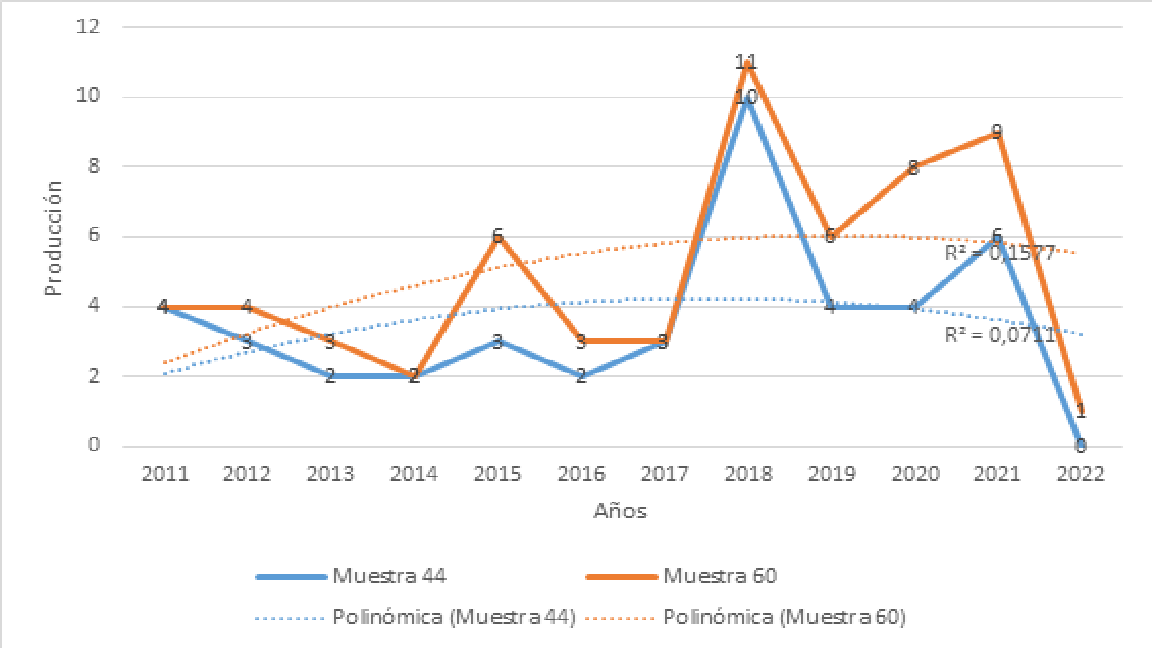
\includegraphics[width=0.85\textwidth]{Fig1.png}
 \caption{Annual scientific production.}
 \label{fig01}
 \source{Elaborated by the author (2022).}
\end{figure}

The previous figure shows the diachronic development of the general topic of neurodidactics of the two samples of scientific documents in which a very similar evolution is observed and whose growth is manifested in a linear manner following \posscite{price_autoradiographic_1973} Law of Logistic Growth of science. This fact is reaffirmed in both cases when adding, in this case, the trend line of polynomial type of degree 2 by calculating its coefficient of determination (R${^2}$) which for the sample of 60 documents yields a value of 0.1577, and for the sample of 44 documents its value is 0.0711. Similarly, Pearson's correlation coefficient (\textit{r}) is calculated, where the value for the sample of 60 documents is 0.34 and for the sample of 44 documents it would be 0.14. In both cases, although there is a positive correlation between time and document production, the correlation values are very low and fall far short of the value of 1, which would be the perfect fit to the model.  

\subsection{Main sources of information}

\Cref{Table02} shows the most relevant sources of information for each of the samples studied in terms of the production of scientific documents.

\begin{table}[h!]
\centering
\caption{Most relevant sources of information.}\label{Table02}
\begin{tabular}{lcc}
\toprule
Fuentes de información & Producción muestra 60 & Producción muestra 44 \\
\hline
Revista Iberoamericana de Educación & 8 & 8 \\
Information Technologies and Learning Tools & 2 & 2 \\
Mathematics & 2 & 0 \\
Revista de Educación Inclusiva & 2 & 2 \\
Revista Inclusiones & 2 & 0 \\
Revista San Gregorio & 2 & 0 \\
\hline
\end{tabular}
\source{Elaborated by the author (2022).}
\end{table}

It is observed that, due to the fact that we do not have very large samples, the number of information sources, as well as the production index of each of the sources, is not very high. In addition, we found that all the sources of information with the highest production correspond to academic journals, although we also found a significant number of proceedings from prestigious international congresses.

In both cases, the \textit{Revista Iberoamericana de Educación} leads with the highest number of articles produced in both samples. The journals \textit{Information Technologies and Learning Tools} and \textit{Revista de Educación Inclusiva} also coincide in both samples with a production of two articles. The other three remaining journals would have produced another two articles in the case of the sample of 60 but none for the sample of 44. The rest of the information sources that do not appear in the table have produced only one scientific document.

\subsection{Most relevant authors}

\Cref{Table03} shows the list of the most relevant authors according to the number of scientific papers produced for both samples.  

\begin{table}[h!]
\centering
\caption{Most relevant authors.}\label{Table03}
\begin{tabular}{lcc}
\toprule
Autores & Producción muestra 60 & Producción muestra 44 \\
\hline
Sabitzer B & 11 & 10 \\
Calle-Alonso F & 2 & 2 \\
Krohn C & 2 & 2 \\
Sánchez-Gómez JM & 2 & 2 \\
Vega-Rodríguez MA & 2 & 2 \\
\hline
\end{tabular}
\source{Elaborated by the author (2022).}
\end{table}

In both cases, Sabitzer B, following the classification of authors of the inverse quadratic law proposed by \textcite{lotka_frequency_1926}, would be the only author considered as a large producer, having 10 or more articles to his credit on the topic of neurodidactics. The rest of the authors in the table would be considered medium producers and those who do not appear and whose production is one article would be called small producers since their incursion into the topic is occasional.

\subsection{Keyword co-occurrence analysis}

With the following co-occurrence analysis based on the associated words, we will try to establish the main specific issues surrounding the topic of neurodidactics as well as the possible thematic trends inferred in order to obtain an overview of its conceptual structure. For this purpose, we will consider the totality of the keywords as a whole, that is, combining both the \textit{author's keywords} and the \textit{keywords plus}. We set the minimum number of occurrences of a keyword to a value of 1. Since there is not a large number of keywords in each of the samples, instead of keeping those with the highest values of occurrences, we will consider all the keywords and then focus on the main relationships and links that can be established, as well as the most relevant research foci. Thus, from the sample of 60 articles we obtain a total of 207 keywords that reach the threshold of at least 1 occurrence, although the largest set of connected elements consists of 192 keywords. On the other hand, we also set a minimum value of 1 in the number of occurrences of a keyword for the sample of 44 scientific papers. Thus, we obtain a total of 150 keywords that reach this threshold, although 146 keywords make up the largest set of connected items (\Cref{fig02}, \Cref{fig03}).

\begin{figure}[htbp]
 \centering
 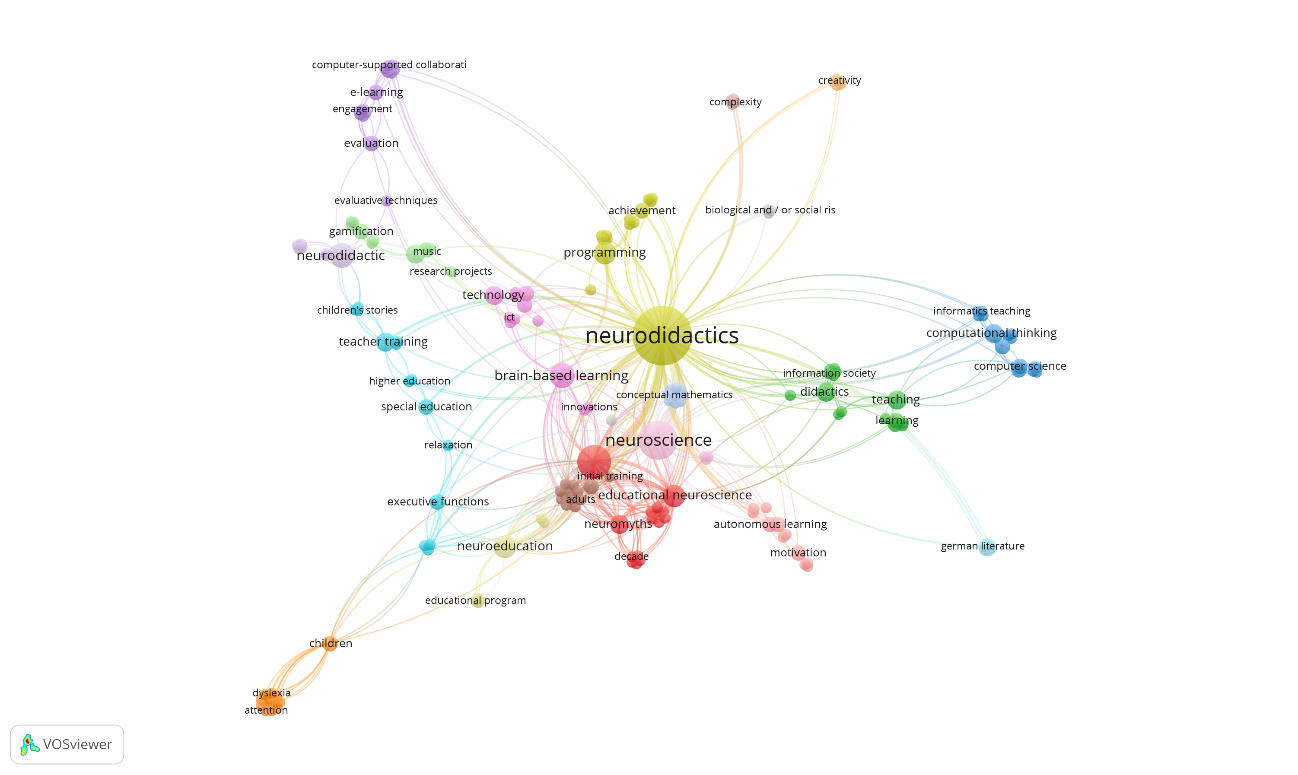
\includegraphics[width=0.85\textwidth]{Fig2.png}
 \caption{Co-occurrence network map of all keywords in the sample of 60.}
 \label{fig02}
 \source{Elaborated by the author (2022).}
\end{figure}

\begin{figure}[htbp]
 \centering
 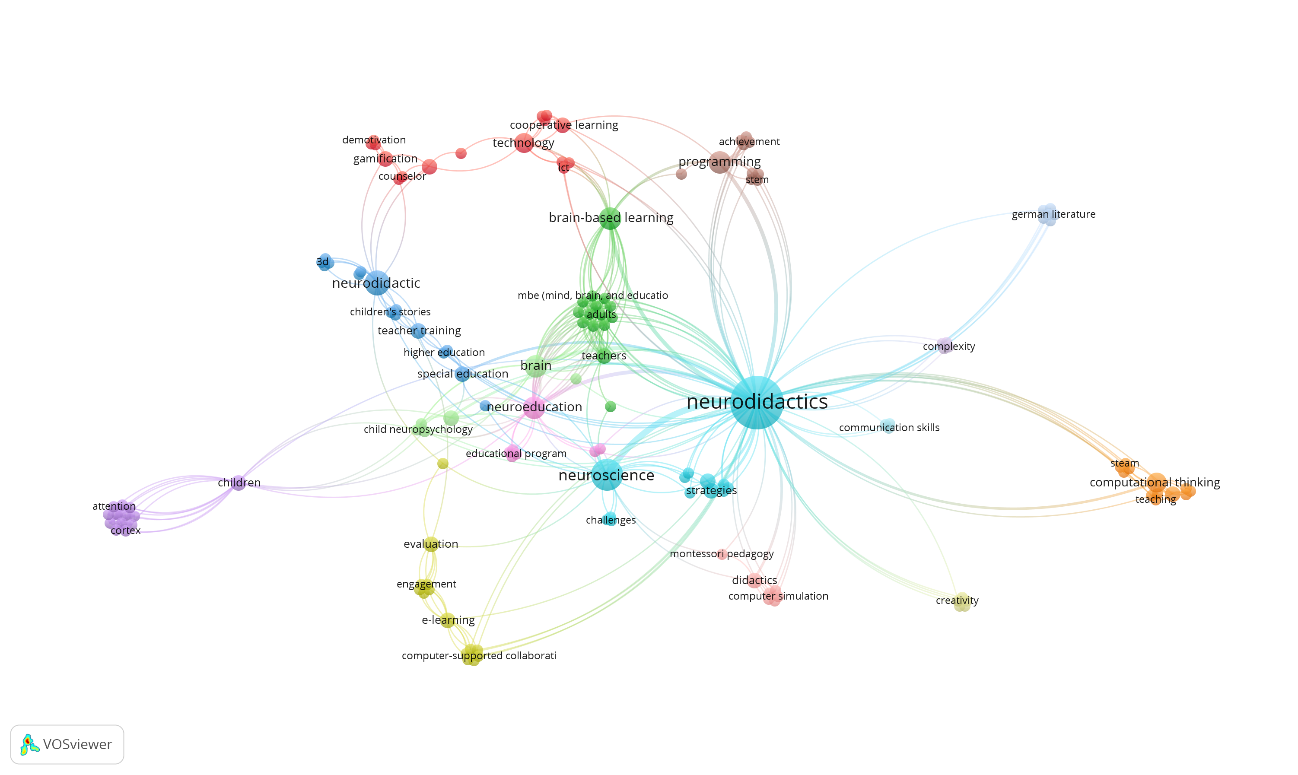
\includegraphics[width=0.85\textwidth]{Fig3.png}
 \caption{Net Network map of co-occurrence of all keywords in the sample of 44.}
 \label{fig03}
 \source{Elaborated by the author (2022).}
\end{figure}

The network maps are presented considering the method of strength of association between their different keywords and showing the strongest links between terms that can be observed by the size and thickness of both the nodes and the links. The different clusters that emerged can be differentiated by colors, although in the comparison between both maps the differences are minimal between the sample of 60 that contemplates different research areas and the sample of 44 focused on educational research areas. The different sizes of the nodes, as well as their names and label sizes indicate whether the occurrence value of a keyword is higher or lower. Each of these nodes can be considered a hot topic that represents a specific problem or a thematic trend within the topic of neurodidactics. Thus, the set of nodes that make up the same cluster identified by a certain color would be determining a general research front according to the nature of each of the keywords that make it up.  Therefore, for the network map composed by the sample of 60 scientific papers, we can infer some research fronts which are more related to the studied topic. We found the yellow research front of neurodidactics, which in turn is the hot topic par excellence, being the most related to the rest of neighboring nodes and clusters, considered as a measure of very high centrality and especially related to the topics \textit{achievement} and \textit{programming}. Another research front to be highlighted is the pink one about neuroscience and technology with relevant terms such as \textit{innovations}, \textit{ict}, \textit{technology} or \textit{brain-based learning}. Related to this research front we found another neighboring dark blue cluster on technological aspects with keywords such as \textit{informatics teaching}, \textit{computational thinking} or \textit{computer science}.

In the case of the sample of 44 scientific papers, practically the same pattern is followed in the formation of research fronts, and the main problems and thematic trends that arouse the greatest interest in the scientific community are very similar. Nevertheless, some clear aspects can be evidenced that mark this small, more specific difference in favor of educational research itself. Beginning with the neurodidactics research front in light blue, it can be seen that on this occasion the main problems and lines of research are directed towards aspects related to neuroscience and certain challenges (\textit{neuroscience} and \textit{challenges}) that can be inferred to be linked to communication \textit{strategies} and \textit{skills}. There is a stronger link between the terms \textit{neuroeducation} and \textit{educational program}, which would highlight a small research front on neuroeducation programs especially applied in the fields of special education and higher education, as indicated by the existing links with the neighboring dark blue cluster. Another research front of a more educational nature that would unite pedagogy and neurodidactics would be the one composed of pink terms such as \textit{didactics}, \textit{computer simulation} and \textit{montessori pedagogy}.

Next, and in an attempt to show in a clearer and more visual way, the strongest links and all the keywords that make up both samples are presented by means of density maps (\Cref{fig04} and \Cref{fig05}). In these maps, the areas colored in yellow coincide with the most important links in the network maps. However, the absence of some areas colored in darker orange or red tones indicates that there is no research front, hot topic, thematic trend or specific problem sufficiently developed to stand out from the rest due to a special interest of the scientific community and that has resulted in a greater and considerable production of scientific papers.

\begin{figure}[htbp]
 \centering
 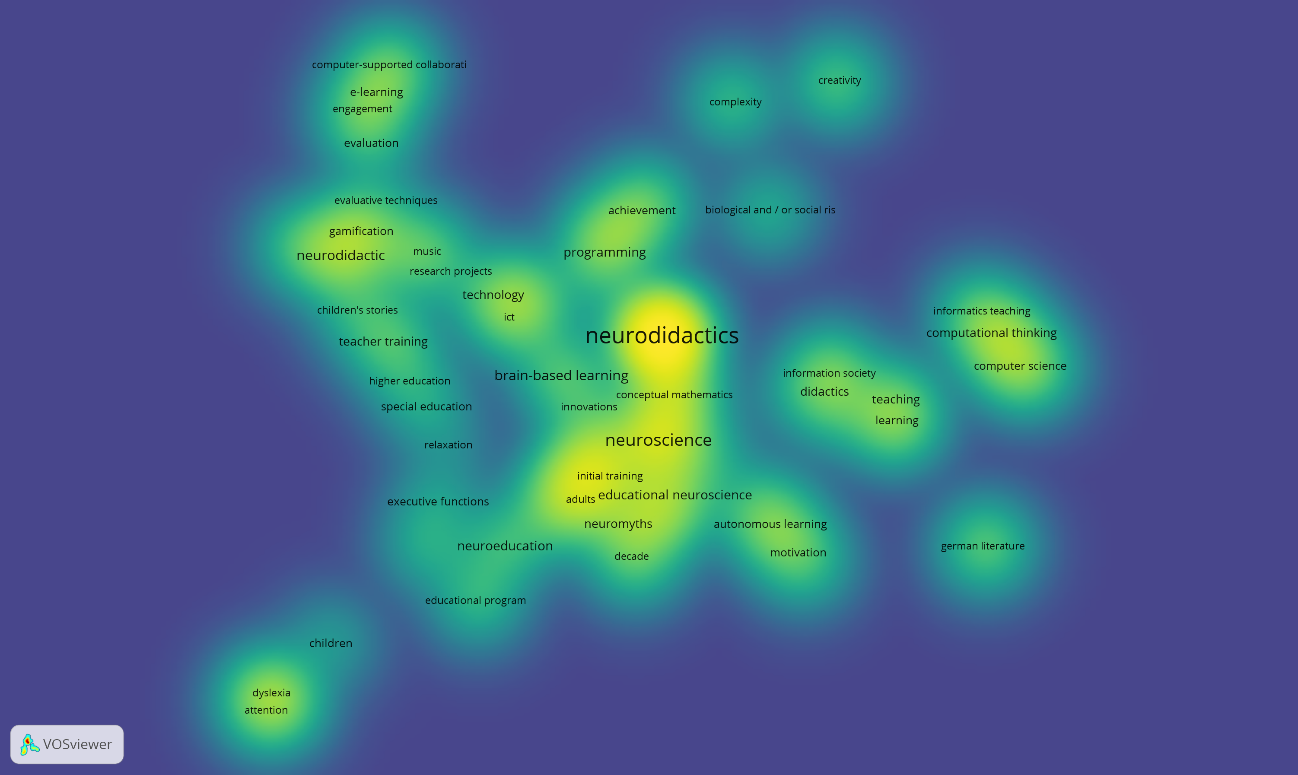
\includegraphics[width=0.85\textwidth]{Fig4.png}
 \caption{Density map of all keywords in the sample of 60.}
 \label{fig04}
 \source{Elaborated by the author (2022).}
\end{figure}

\begin{figure}[htbp]
 \centering
 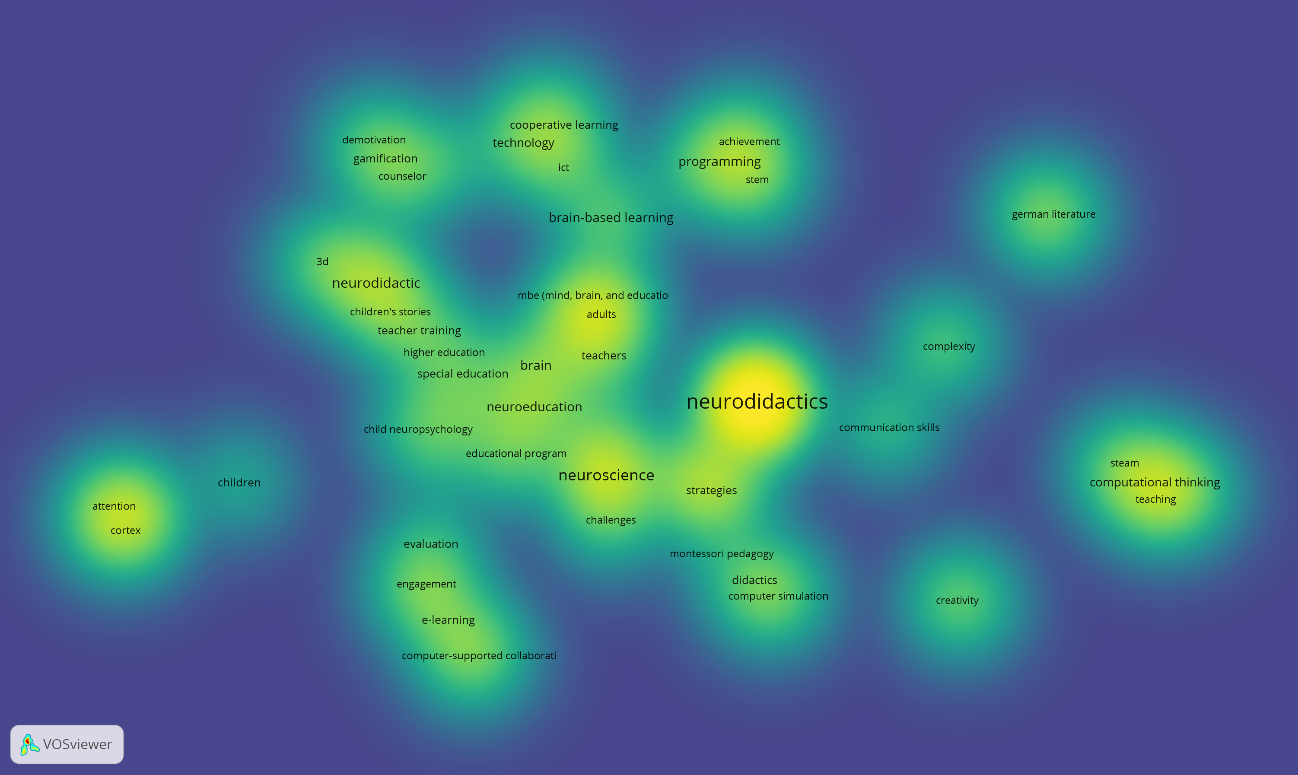
\includegraphics[width=0.85\textwidth]{Fig5.png}
 \caption{Density map of all the keywords in the sample of 44.}
 \label{fig05}
 \source{Elaborated by the author (2022).}
\end{figure}

\section{Discussion and conclusions}

One of the most useful tools that we have been able to use in our research at the present time is precisely quantitative-bibliometric studies, with the intention of measuring the results of the research activity of different authors or the scientific activity of some journals. The objective is to be able to understand and objectify some of the facts that may occur in the scientific field. We are aware of the difficulty involved in some more educational investigations, being able to change the results of any investigation, depending on cultural, economic and political facts.

If as trainers in higher education we want to understand and deepen learning in adulthood, knowledge of neurosciences will be necessary \cite{campos_neuroeducacion:_2010,codina_felip_neuroeducacion_2015,barrios_tao_neurociencias_2016}, in order to be able to explain and understand all the complexity in the construction of mental processes, thus improving learning skills and knowledge that are more relevant to the development of our society.

One of the key factors will necessarily be linked to the knowledge of neurodidactics \cite{fernandez_palacio_neurodidactica_2017,benavidez__importancia_2019,eyzaguirre_estrategia_2020}, in order to select the most appropriate forms of innovative and methodological approaches inside and outside the classroom. Together with what was mentioned in the previous paragraph, the use of Information and Communication Technologies (ICT) will serve as a means of support for learning in adulthood, taking into account the enormous plasticity of the brain throughout the life of the human being.

From the methodological planning of this article, in its second part, we presented an investigation with a general structure of the development of the topic of neuroscience and its main relationship with information and communication technologies, education and teaching from its bibliometric analysis. According to the results obtained, at the level of diachronic production in both samples, this is an area of study that has not found its level of logistic stabilization proposed by \textcite{price_autoradiographic_1973}, i.e., it is not a fully mature discipline and it is expected that its production will continue to grow over time. Therefore, the rest of the analyses have yielded results that have been shown to be in line with this fact. So far, few sources of information have been published on this topic. In fact, although many of these sources are proceedings of prestigious international congresses such as ICERI or INTED, among others, as far as academic journals are concerned they do not stand out for their high citation impact or for being indexed in databases of great recognition among members of the scientific community. Following this dynamic, we find that, except for the author Sabitzer B, there are no authors who are experts in the subject and who have a long history of study and research on the topic. Although following the distribution of authors such as \textcite{lotka_frequency_1926}, others who have appeared in this study have been considered as incipient producers, the truth is that all of them do not exceed two contributions to the field studied.

As for the co-occurrence analysis based on the keywords of the scientific papers, a series of network and density maps are generated where the main thematic links are observed. From the observation of these maps, a total of five research fronts have been inferred as the most relevant and related to the topic such as: neurodidactics in general; neuroscience and technology; neurodidactics and technological aspects; neuroeducation programs and; pedagogy and neurodidactics \cite{_nieto_bases_2014}. As this is a developing field of study, no major specific problems have been found, but for the time being what was obtained is a broad and general view of this area of research.

Future works that complements or expands this study could be oriented towards carrying out replication studies but increasing the time spectrum to observe possible variations in the growth or not of scientific production, as well as considering other indicators to obtain more information about its intellectual structure, such as an analysis of co-citation among authors, or its social structure in which to identify the most productive countries and/or institutions as well as to analyze the rate of collaboration between these countries or academic institutions.  

\printbibliography\label{sec-bib}
% if the text is not in Portuguese, it might be necessary to use the code below instead to print the correct ABNT abbreviations [s.n.], [s.l.]
%\begin{portuguese}
%\printbibliography[title={Bibliography}]
%\end{portuguese}


%full list: conceptualization,datacuration,formalanalysis,funding,investigation,methodology,projadm,resources,software,supervision,validation,visualization,writing,review
\begin{contributors}[sec-contributors]
\authorcontribution{Borja Fernández García-Valdecasas}[conceptualization,formalanalysis,methodology,validation,writing,review]
\authorcontribution{Isabel Martínez Sánchez}[conceptualization,formalanalysis,methodology,validation,writing,review]
\authorcontribution{Daniel González González}[conceptualization,formalanalysis,methodology,validation,writing,review]
\authorcontribution{José Álvarez Rodríguez}[conceptualization,formalanalysis,methodology,validation,writing,review]
\end{contributors}

\end{document}